\documentclass[a4paper,12pt]{article}

\title{Programmering og Problemløsning, ugeseddel 2}
\author{Version 1.3}% Torben Mogensen, Martin Dybdal og Hans J. T. Stephensen
\date{8.\ September 2015}

\usepackage[top=2cm,left=25mm]{geometry}
\usepackage[T1]{fontenc}
\usepackage[utf8]{inputenc}
\usepackage[danish]{babel}
%\usepackage{microtype}
\hyphenpenalty=750

\usepackage{amsmath}
%\usepackage{lmodern}
%\usepackage{mathptmx}
%\usepackage{libertine}
%\usepackage[scaled=0.90]{inconsolata}
%\usepackage[scaled=0.83]{beramono}

\usepackage{enumerate}
\usepackage{listing}
\usepackage{fancyvrb}
\usepackage{graphics,tikz}

\usepackage{todonotes}


\usepackage{hyperref}
\hypersetup{pdftitle={Programmering og Problemløsning, ugeseddel 2},
            pdfsubject={},
            pdfauthor={},
            pdfkeywords={rekursion, funktioner, lister, sæt},
            pdfborder={0 0 0}}

\setlength{\parskip}{1ex}
\setlength{\parindent}{0pt}
\setlength{\parfillskip}{30pt plus 1 fil}

\newcommand{\fs}{\texttt{F\#} }
\newcommand{\fsi}{\texttt{F\# Interactive} }


\begin{document}
\maketitle{}

Den anden undervisningsuge har til formål at gøre dig fortrolig med
programmering i \fs med brug af tupler (sæt) og lister.

Der er i uge 2 en obligatorisk opgave, som består af en
gruppeopgave og en individuel opgave.


\section{Pensum og plan for ugen}
\label{sec:pensum-og-plan}


\textbf{Pensum for uge 2:} HR afsnit 3.3 samt kapitel 5 og 6.  IP-2
afsnit 4.3--4.4, 4.6 (undtagen 4.6.1), 4.7, 5.1--5.4, 5.6, kapitel 6,
afsnit 7.2--7.4.1.  Noterne ``Hvordan man angriber et
programmeringsproblem'' og ``Vejledning om test'' (findes under
``Undervisningsmateriale'' på Absalon).

\textbf{Foreslået læserækkefølge:} HR afsnit 3.3, IP-2 afsnit
4.3--4.4, 4.6, 5.1--5.4, 5.6, ``Vejledning om test'', HR kapitel 5,
IP-2 kapitel 5, HR kapitel 6, ``Hvordan man angriber et
programmeringsproblem'', (til fredag) IP-2 afsnit 7.1--7.4.1.

Forelæsningen mandag 8:15 -- ca.\ 8:50 repeterer stoffet fra uge 1.
Forelæsningen 09:00--10:00 vil fokusere på tupler (sæt), polymorfi og
afprøvning.  Øvelserne vil omhandle det samme og inddrage elementer
fra uge 1.

Tirsdag omhandler både forelæsninger og øvelser lister samt
systematisk problemløsning.

Forelæsningen fredag omhandler køretid.  Øvelserne bruges til at
arbejde med den individuelle opgave.


%\newpage
\section{Mandagsopgaver}
\label{sec:mandagsopgaver}

Mål: Fortrolighed med selekteringsfunktioner, erklæring af infix
operatorer samt systematisk afprøvning.

\begin{enumerate}[{2}M1]
\item HR opgave 3.3 (a) og (b).  Lav test som beskrevet i ``Vejledning
  om test''. \textbf{Vink:} Se prædefinerede operator præcedens på side
  316 i HR.
\item IP-2 opgave 4.1 og 4.4.  Lav test som beskrevet i ``Vejledning
  om test''.
\item Omskriv gcd-funktionen fra side 26 i HR (den, der bruger
  if-then-else), så den tager ét argument \texttt{mn} af typen
  \texttt{int\,*\,int} og bruger selektionsfunktionerne \texttt{\#1}
  og \texttt{\#2} til at tilgå komponenterne i parret \texttt{mn}.
  Vurder læseligheden af programmet sammenlignet med de versioner af
  gcd, der er vist på side 20 og 26 i HR.
\item IP-2 opgave 4.6.
\end{enumerate}


%\newpage
\section{Tirsdagsopgaver}
\label{sec:tirsdagsopgaver}

Mål: Programmering med lister og systematisk problemløsning.

Det forventes, at du inden øvelserne tirsdag har forberedt dig på
opgaverne ved at løse så mange som muligt på egen hånd.

\begin{enumerate}[{2}T1]
 \item HR opgave 5.2, 5.3, og 5.7.
 \item I ASCII alfabetet (HR side 346 og IP-2 side 17) kommer alle de
   store bogstaver før alle de små bogstaver, så sammenligningen
   \texttt{"XYZ"\,<\,"abc"} giver værdien \texttt{true}, hvilket ikke
   er konsistent med den måde, man ordner ord i en ordbog.

\begin{enumerate}[(a)]

   \item Beskriv i tekst, hvordan ord er ordnet i en ordbog.

   \item Beskriv i tekst en plan for, hvordan man kan implementere
     denne ordning i \fs og beskriv et antal tests, der med rimelighed
     kan overbevise en læser om, at denne funktion fungerer rigtigt.
     Tænk over specialtilfælde, og overvej, om der er funktioner i
     modulerne \texttt{Char} og \texttt{String} (Appendix D3 i HR),
     som kunne være brugbare til at løse problemet.  Du behøver ikke
     at tage hensyn til danske bogstaver (æ, ø og å), accenter eller
     til rækkefølgen af ikke-alfabetiske tegn i ordbøger, og ejheller,
     at aa nogen gange alfabetiseres efter z.  Med andre ord, er det
     kun ord, der er bygget af bogstaverne a til z og A til Z, du skal
     kunne teste for ordbogsorden.

   \item Skriv i \fs en funktion
     \texttt{ordbogsOrden\,:\,string\,*\,string\,->\,bool}, sådan at
     kaldet \texttt{ordbogsOrden ($p$,$q$)} giver \texttt{true}, hvis
     ordet $p$ kommer før ordet $q$ i ordbogsordenen.

   \item Udfør den planlagte test og reflekter over resultatet.  Blev
     der fundet fejl? Var der flere ting, man med rimelighed havde kunnet
     afprøve?

   \item Reflekter over processen og resultatet: Havde det hjulpet at
     bruge mere tid i de første faser?  Kan funktionen programmeres
     pænere?

  \end{enumerate}
\item HR opgave 5.17

\end{enumerate}

\newpage
\section{Opgavetema: Geografiske koordinater}
Den præcise angivelse af et punkt på jordens overflade kan defineres
ud fra en \textit{breddegrad}, der angiver hvor langt mod syd eller
nord punktet er i forhold til ækvator, og en \textit{længdegrad}, der
angiver hvor langt øst/vestligt punktet er i forhold til \textit{Royal
  Observatory Greenwich} i London.

De to tal opgives i et antal grader: En breddegrad er et
\textit{reelt} tal mellem $-90.0^\circ$ (Sydpolen) og $90.0^\circ$
(Nordpolen), og en længdegrad er et \textit{reelt} tal mellem
$-180.0^\circ$ og $180.0^\circ$. Breddegraden $0.0^\circ$ er ved
ækvator, og længdegraden $0.0^\circ$ er ved føromtalte observatorium.

I \fs kan vi altså definere et sådant geografisk koordinat som et par
af to reelle tal (breddegrad og længdegrad).  F.eks.\ kan vi definere
koordinaterne til Universitetsparken 1 og koordinaterne til
Peterskirken i Rom:
\begin{verbatim}
>let diku_up1 = (55.702028, 12.561144);;
val diku_up1 : float * float = (55.702028, 12.561144)
>let peterskirken = (41.902139, 12.453336);;
val peterskirken : float * float = (41.902139, 12.453336)

\end{verbatim}
For at verificere et koordinat kan i taste det ind på formen
"`55.702028, 12.561144"' i søgefeltet på Google Maps
(\url{http://maps.google.dk}). Med Google Maps kan I også aflæse andre
koordinater ved at højreklikke og vælge "`Hvad er der her?"' eller
"`What's here?"' i den engelsksprogede udgave. At udvælge jeres egne
koordinater på denne måde kan være anvendeligt når I skal skrive
afprøvning af jeres funktioner.

\begin{center}
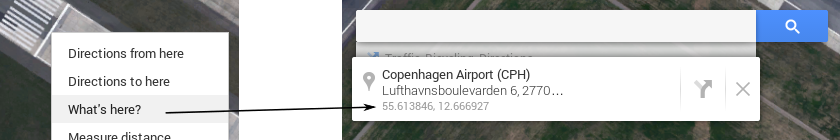
\includegraphics[width=0.8\textwidth]{uge2_googlemaps.png}
\end{center}


Desværre er jorden ikke flad, og derfor er det ikke helt så simpelt at
beregne afstande mellem to punkter på jordoverfladen, da man skal tage
højde for jordens krumning og det noget anderledes koordinatsystem.  Vi
udleverer derfor en funktion, der kan beregne afstande (i kilometer),
som I skal bruge til de efterfølgende opgaver. Funktionen hedder
\verb|distance| og findes i filen \texttt{uge2\_distance.fsx}, der
ligger sammen med ugesedlen på Absalon. I kan enten kopiere indholdet
ind i jeres aflevering eller tilføje en \verb|use|-erklæring i starten
af filen:
\begin{verbatim}
#load "uge2_distance.fsx";;    (* Husk semikolonnet! *)
\end{verbatim}
For at finde afstanden (kilometer i fugleflugt) mellem
Universitetsparken 1 og Peterskirken skrives:
\begin{verbatim}
> Uge2Dist.distance diku_up1 peterskirken;;
val it : float = 1534.497475
\end{verbatim}
I må ikke blive bange for at bruge den slags funktioner i ikke helt
forstår. Dataloger vil altid skulle arbejde tæt sammen med andre
specialister. I skal vænne jer til at man ikke behøver at forstå,
hvordan alle dele af et program helt konkret er sat sammen, når man
bare kan forstå, hvad de gør (og stoler på at de gør det der er blevet
lovet).

%\newpage
\section{Gruppeaflevering}
\label{sec:gruppeaflevering}
I uge 2 og fremover er gruppeafleveringen obligatorisk.  Alle
delspørgsmål skal besvares.  Opgaven afleveres i Absalon.  Der
afleveres en fil pr.\ gruppe, men den skal angive alle deltageres
fulde navne i kommentarlinjer øverst i filen. Filens navn skal være af
formen \texttt{2G-\textit{initialer}.fsx}, hvor initialer er erstattet
af gruppemedlemmernes initialer. Hvis f.eks. Bill~Gates,
Linus~Torvalds, Steve~Jobs og Gabe~Logan~Newell afleverer en opgave
sammen, skal filen hedde \texttt{2G-BG-LT-SJ-GLN.fsx}. Brug
gruppeafleveringsfunktionen i Absalon.

Gruppeopgaven giver op til 2 point, som tæller til de 20 point, der
kræves for eksamensdeltagelse.  Genaflevering kan hæve pointtallet fra
første aflevering med højest 1 point, så sørg for at gøre jeres bedste
allerede i første aflevering.

\textbf{NB!} Der skal laves systematisk afprøvning af alle opgaverne i
gruppeopgaven jvf.\ noten ``Vejledning i test''.

\begin{enumerate}[{2}G1]
\item En løberute kan beskrives som en liste af koordinater, hvor det
  første er start-koordinatet, og det sidste er endepunktet på
  ruten.  Vi har vedlagt en rute i dette format i filen
  \texttt{uge2\_cphmarathon2014.fsx}:
  \begin{verbatim}
  let cphMarathon2014 = [(55.66639000,12.57621000),
                         (55.66794000,12.57822000),
                         (55.66858000,12.57914000),
                         ...
                         (55.66659000,12.57647000)];\end{verbatim}
  Skriv en funktion der måler den samlede afstand af ruten (i
  kilometer) vha. \verb|distance|-funktionen beskrevet
  ovenfor. Funktionen skal have følgende typesignatur:
  \verb| totalDistance : (float * float) list -> float|

  Maratonruten er ikke helt nøjagtigt målt op af løberen, så i stedet
  for de $42,195$ kilometer som maratondistancen er defineret til, skal I
  forvente følgende svar. I kan se bort fra afvigelser på de sidste
  decimaler.
\begin{verbatim}
> totalDistance cphMarathon2014;
val it : float = 42.9686446838
\end{verbatim}
\item Når en løberute optages med et løbeur eller mobiltelefon med
  GPS-enhed gemmes ikke kun koordinaterne, men også tidspunkt.  I
  vores repræsentation er et tidspunkt repræsenteret som et helt antal
  millisekunder siden starten af løbet.  Vi har som eksempel vedlagt
  en rute med angivet tid i filen \verb|uge2_dhl2014.fsx|.  Denne
  definerer en variabel \verb|dhl2014 : ((float * float) * int) list|,
  hvor parret af kommatal er GPS-koordinaterne og heltallet er
  antallet af millisekunder siden start.  Det første punkt på ruten er
  startpunktet, som følgelig har tiden 0.

  Skriv en funktion der beregner hastigheden (i km/t) på hvert segment
  af en rute:

  \verb|  speeds : ((float * float) * int) list -> float list|

  Bemærk, at den resulterende liste er et element kortere end
  inddatalisten, da en sekvens af $n$ punkter har $n-1$ mellemliggende
  segmenter.  Hvis inddatalisten er tom, rejses undtagelsen
  \verb|Empty|.

  \textit{Eksempel:} Hængebroen over Storebælt er ca. 6,8 km lang,
  hvis en løber skal løbe frem og tilbage over broen og han på vejen
  frem bruger 25 minutter (1500000 millisekunder) og på vejen tilbage
  bruger 35 minutter (2100000 millisekunder), vil datasættet se
  således ud (hvis løbeuret kun har registreret koordinater og tid i hver ende af
  broen):
\begin{verbatim}
  let storebaelt = [((55.336145, 10.990714), 0);
                    ((55.349420, 11.095690), 1500000);
                    ((55.336145, 10.990714), 3600000)]
\end{verbatim}
Gennemsnitshastigheden på hver af de to segmenter skal kunne
beregnes til cirka:
\begin{verbatim}
> speeds storebaelt;
val it : float list = [16.3201496895; 11.6572497782]
\end{verbatim}

\item Skriv en funktion der returnerer gennemsnittet af tallene i en
  liste.  Funktionen skal have følgende typesignatur:
  \verb|averageAll : float list -> float|. Hvis listen er tom rejses
  undtagelsen \verb|Empty|.

\item Brug funktionerne \verb|speeds| og \verb|averageAll| til at
  definere en funktion

  \verb|  averageSpeed : ((float * float) * int) list -> float|

  som finder gennemsnitshastigheden for en rute.  Hvis ruten er tom,
  rejses undtagelsen \verb|Empty|.  Hvis ruten kun har et punkt,
  rejses undtagelsen \verb|Domain|.

  Forvent en gennemsnitshastighed på ca. 13.988 km/t for
  Storebælts-eksemplet.

\item Når jeres instruktor retter jeres opgaver, kommenterer de på
  blandt andet følgende punkter:

\begin{itemize}

\item Er funktionen korrekt: Har den den type, som opgaven krævede, og
  gør den det, der er krævet i opgaven?

\item Er funktionen skrævet på en pæn og læselig måde: Er indrykningen
  passende, er der et passende omfang af informationsbærende
  kommenterarer?  Er der ting, der kunne gøres enklere? Er der brugt
  fornuftig navngivning for funktioner og variabel navne.

\item Tester afprøvningen alle relevante tilfælde uden at have
  overflødige testtilfælde?
\end{itemize}

Som svar på opgave 1I3 fra ugeseddel 1, har en elev indleveret
følgende besvarelse:
{\footnotesize
\begin{Verbatim}
(* hvis længden af s er w, returneres s, *)
(* ellers sættes et blanktegn foran, og der kaldes rekursivt *)
fun rightAlignHelper (s, w) = if String.size s = w then s else rightAlignHelper (" " ^ s, w)
(* Konverter tallet n til tekst og tilføj blanktegn foran, *)
(* indtil længden er w *)
fun rightAlign (n, 0) = raise Domain
  | rightAlign (n, w) = rightAlignHelper(Int.toString n, w)

val test_rightAlign1 = rightAlign(17,4) = "  17"
val test_rightAlign2 = rightAlign(~17,4) = " ~17"
\end{Verbatim}
}

Bedøm denne besvarelse ud fra de ovennævnte kriterier.  Giv både ris
og ros.  Skriv jeres bedømmelse som en kommentar i den afleverede
\verb|.fsx| fil.

\end{enumerate}

%\newpage
\section{Individuel aflevering}
\label{sec:indiv-aflev}

Også den individuelle opgave er obligatorisk i uge 2 og fremover.
Alle delspørgsmål skal besvares.  Opgaven afleveres i Absalon som en
fil med navnet \texttt{2I-\textit{navn}.fsx}, hvor
\texttt{\textit{navn}} er erstatttet med dit navn. Hvis du fx hedder
Anders~A.~And, skal filnavnet være \texttt{2I-Anders-A-And.fsx}. Skriv
også dit fulde navn som en kommentar i starten af filen.

Den individielle opgave giver op til 3 point, som tæller til de 20
point, der kræves for eksamensdeltagelse.  Genaflevering kan hæve
pointtallet fra første aflevering med højest 1 point, så sørg for at
gøre dit bedste allerede i første aflevering.

Den individuelle opgave i denne uge fortsætter temaet om
GPS-koordinater fra ugens gruppeopgave.

\textbf{NB!} Der skal også i den individuelle aflevering laves
systematisk afprøvning af alle opgaverne jvf.\ noten ``Vejledning i
test''.


\begin{enumerate}[{2I}1]

\item I mange GPS-systemer er der mulighed for at finde det nærmeste
  interessepunkt. F.eks. "`Nærmeste benzintank"', "`Nærmeste
  supermarked"'.

  Skriv funktionen:

  \verb|  closestDistance : ((float * float) * (float * float) list) -> float|

  sådan at kaldet \verb|closestDistance p qs| beregner
  \textit{afstanden} til det koordinat i listen \verb|qs| som er
  tættest på koordinatet \verb|p| i fugleflugtslinje.  Hvis listen er tom, rejses
  undtagelsen \verb|Empty|.  Brug denne funktion til at finde den
  korteste afstand fra DIKU (Universitetsparken 1) til et punkt på
  ruten for Københavns maraton.

  Vink: Brug \verb|List.min|.

\item Det er ikke altid man kun er interesseret i afstanden til det
  nærmeste punkt, men også noget information om selve punktet. I filen
  \verb|uge2_kollegier.fsx| har vi vedlagt listen:
  \begin{verbatim}
  let kollegier = [((55.662539, 12.609901), "Frankrigsgadekollegiet");
                   ((55.654295, 12.592202), "Grønjordskollegiet");
                   ((55.700325, 12.553688), "Kollegiegården");
                   ...
                  ]
  \end{verbatim}
  Skriv funktionen:

  \verb|  closestPOI : ((float * float) * ((float * float) * 'a) list) -> 'a|

  der i stedet for at returnere \textit{afstanden} til det nærmeste
  interessepunkt, skal I returnere \textit{beskrivelsen} af
  interessepunktet.

  Vink: Skriv en hjælpefunktion, der returnerer \textit{både}
  koordinatet og beskrivelsen.

\item Bemærk, at typen af beskrivelsen i signaturen for \verb|closestPOI|
  er angivet som \verb|'a| og ikke som \verb|string|.  Forklar i en
  kommentar i din besvarelse, hvorfor dette er tilfældet.

\end{enumerate}

%\newpage
\section{Ugens nød}
\label{sec:ugens-nod}

Ugens nød er en frivillig, særligt udfordrende opgave, der kan løses
af særligt interesserede studerende.  Opgaven kan løses kun ved brug
af begreber, der allerede er undervist i, men kræver ekstra omtanke og
nogen gange en god ide.  Afleveringsfristen er den samme som for den
individuelle opgave.  Ved fredagsforelæsningen i den efterfølgende uge
kåres den bedste løsning til ugens nød, og vinderen får en lille
præmie, typisk et stykke chokolade eller andet guf.

\subsection*{Selvbeskrivende sætninger}

En sætning af formen ``Denne sætning \ldots'' siges at være
selvbeskrivende.  En selvbeskrivende sætning kan være sand (som
f.eks.\ ``Denne sætning indeholder flere end ti tegn'') eller falsk
(som f.eks.\ ``Denne sætning indeholder flere end hundrede tegn'').
Den kan også have udefineret sandhedsværdi (som f.eks.\ ``Denne
sætning er falsk''), men hvis en sætning blot udtaler sig om antallet
af tegn i sig selv, er den klart enten sand eller falsk.

\begin{enumerate}[{2}N1]

\item Lav en funktion \texttt{talord : int -> string}, der tager et
  heltal $0 \leq n < 1000$ og returnerer en tegnfølge, der er talordet
  for $n$.  F.eks.\ skal \texttt{talord 0} returnere tegnfølgen
  \texttt{"nul"} og \texttt{talord 345} skal returnere tegnfølgen
  \texttt{"trehundredefemogfyrre"}.

\item Lav et program \texttt{findSand : unit -> string}, der
  returnerer en sætning af formen \texttt{"Denne sætning indeholder
    præcis $n$ bogstaver."}, hvor $n$ er et talord, og sætningen er
  sand.  Bemærk, at blanktegn og punktum ikke betragtes som bogstaver.
  Vis resultatet af kaldet \texttt{findSand ()}.

\item Lav et program \texttt{findSand2 : unit -> string}, der
  returnerer en sætning af formen \texttt{"Denne sætning indeholder
    præcis $v$ vokaler og $k$ konsonanter."},\newline hvor $v$ og $k$ er
  talord, og sætningen er sand. Vis resultatet af kaldet
  \texttt{findSand2\,()}.

\item Lav et program \texttt{findSand3 : unit -> string}, der
  returnerer en sætning af formen \texttt{"Denne sætning indeholder
    præcis $a$ a'er, et b, et c, $d$ d'er, \ldots, $y$ y'er, et z, tre
    æ'er, et ø og et å."}, hvor $a, \ldots, y$ er talord, og sætningen
  er sand.  Bemærk at, idet talord for tal under 1000 ikke bruger
  alle bogstaver i alfabetet, er nogle af talordene givet på forhånd.
  F.eks.\ vil sætningen altid indeholde et b og tre æ'er.  Bemærk
  også, at der ikke gøres forskel på store og små bogstaver, så
  initialen ``D'' tæller med til d'erne.  Det er endvidere ikke
  korrekt at skrive f.eks.\ ``et a'er'', da det hedder ``et a''.

  Vis resultatet af kaldet \texttt{findSand3 ()}.

\end{enumerate}

Det er ikke sikkert, at nogen finder en helt korrekt løsning, så
præmien gives til den, der finder den løsning, der er korrekt for
flest mulige bogstaver.  Man kan f.eks.\ lave en funktion, der tager
et tal $z$ som ekstra parameter og finder en løsning med mindst $z$
rigtige talord.  Som \emph{tie breaker} bruges en vurdering af, hvor
pænt programmet er skrevet.


\end{document}

%%% Local Variables:
%%% mode: latex
%%% TeX-master: t
%%% End:
